\begin{frame}

\begin{textblock}{1}(13,-3.5)$(15,36)$\end{textblock}

\frametitle{Functions in \D{}}

$$f = \left\langle v, C \right\rangle \quad \text{s.t.} \quad \forall\
\left\langle v',\_,\_ \right\rangle \in C\ \left( v'=v \right)$$

%\vspace{1in}

\begin{center}

Pattern matching is ensured {\bf exhaustive} at compile time, i.e.

$$\forall\ b \in \mathbb{B}\ \exists\ c \in C\ c\succ b.$$

WLOG, $c = \left\langle p,x \right\rangle$.

\end{center}

\end{frame}

\begin{frame}[fragile]

\begin{textblock}{1}(13.8,-3.5)$(15)$\end{textblock}

\frametitle{Patterns and shapes}

\begin{columns}
\column{0.5\textwidth}
\begin{center}
\mono{f (\_.0).0 := ...}
\end{center}

\column{0.5\textwidth}
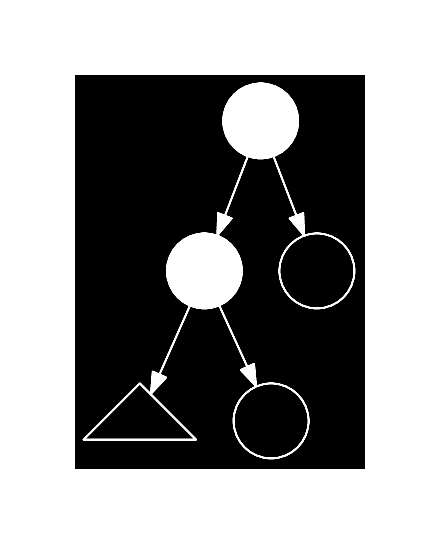
\includegraphics[scale=0.5]{figures/shape}

\end{columns}

\end{frame}

\begin{frame}[fragile]

\begin{codebox}
\Procname{$\proc{Ensure-Exhaustive}(c : C)$}
\li $P_{siblings} \gets \proc{Get-Siblings}(c)$
\li $C' \gets [c]$
\li \For $c'\in C$ \Do
\li $(P_{success},P_{fail}) \gets \proc{Match-Clause-To-Siblings}(c,P_s)$
\li \For $p\in P_{success}$ \Do
\li $c'' \gets \proc{Clone}(c')$
\li $\proc{Merge-Pattern}(c'',p)^{\color{green}\textt{\bf *}}$
\li $C' \gets c' : C'$ \End
\li $P_{siblings} \gets P_{fail}$ \End
\li \Return $C'$
\end{codebox}

{\bf Invariants:}

\begin{itemize}

\item \bi $P_{siblings}$ is always a list of siblings that wasn't matched by
any forthcoming clause.

\item \bi $P_{success}$ and $P_{fail}$ are always sibling lists.

\end{itemize}

\end{frame}

\begin{frame}

$$S_1\Cup S_2 = \left\{ s \left|
\begin{array}{ll} &\left(s\in S_1 \wedge \left(\exists\ s_2\in S_2\ s\cap
s_2\neq\emptyset \longrightarrow s\succ s_2 \right) \right)\\ \vee & \left( s\in
S_2 \wedge \left(\exists\ s_1\in S_1\ s\cap s_1\neq\emptyset \longrightarrow
s\succ s_1 \right) \right) \end{array} \right.\right\}$$

\vspace{0.5in}

\begin{center}

There's a small detail missing\ldots

\end{center}

\end{frame}
